
\chapter{Results}

\acresetall


\section{Humanly Perceived Improvement vs. Machine Performance}


\subsection{Investigating Existing Data}

The direct comparison method outlined in \subsecref{Method-Existing-Data}
was carried out on the data given in \secref{litresults} \textit{\nameref{sec:litresults}}.
The R code used to perform this analysis is given in \lstref{directComp}.

\figref{Direct-PESQ-PRR} shows the results obtained, comparing the
\ac{PESQ} improvement against the \ac{PRR} improvement. \figref{Direct-PESQ-PRR-LOESS}
shows the data fitted with an \ac{LOESS} model and \figref{Direct-PESQ-PRR-LM}
shows the data fitted with an \ac{LM} method.

\begin{figure}[p]
\subfloat[\label{fig:Direct-PESQ-PRR-LOESS}\acs{LOESS} fit]{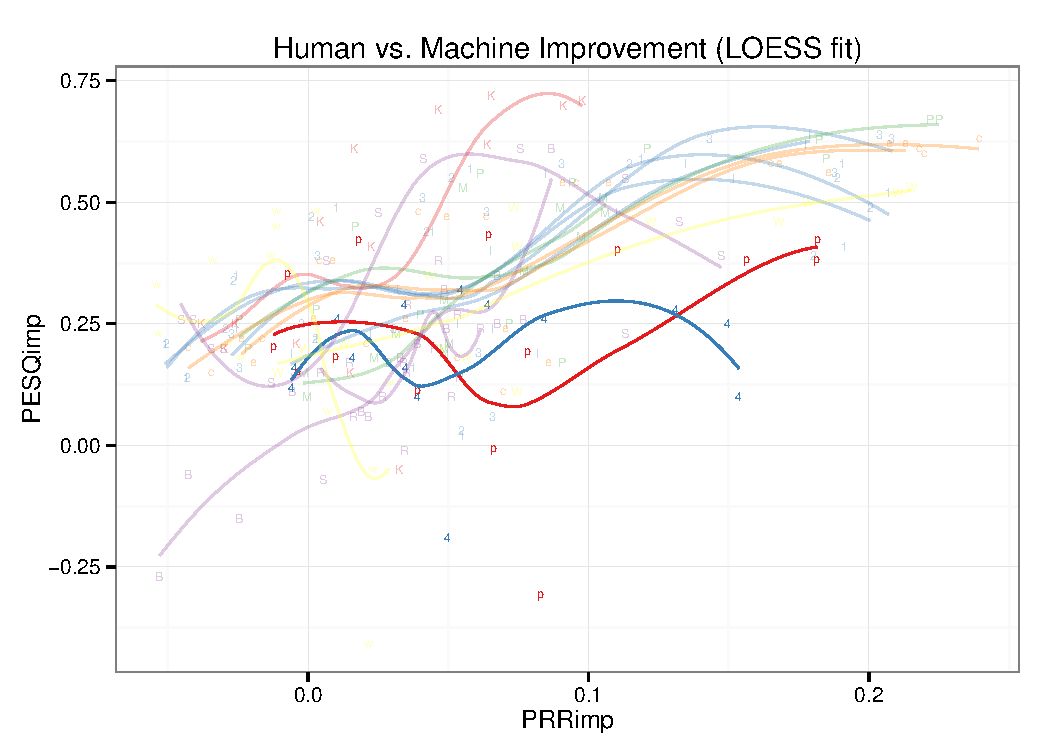
\includegraphics[width=1\textwidth]{fig/R/dir/lit/HumanMachineAllLOESS}

}

\subfloat[\label{fig:Direct-PESQ-PRR-LM}\acl{LM} fit]{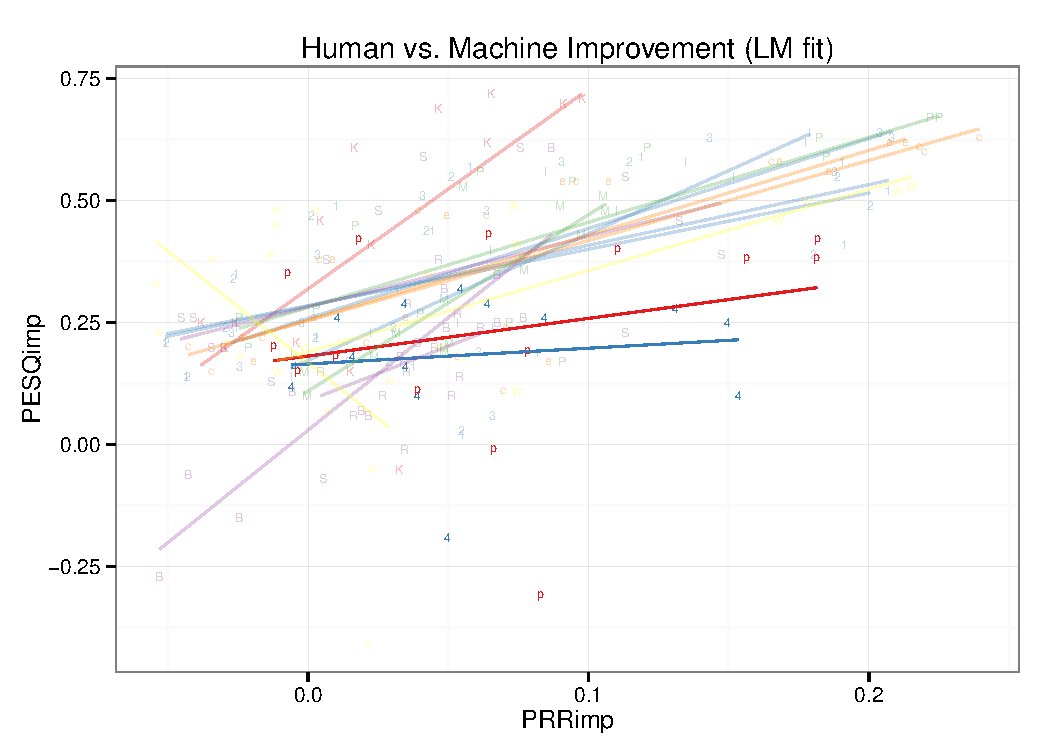
\includegraphics[width=0.8\textwidth]{fig/R/dir/lit/HumanMachineAllLM}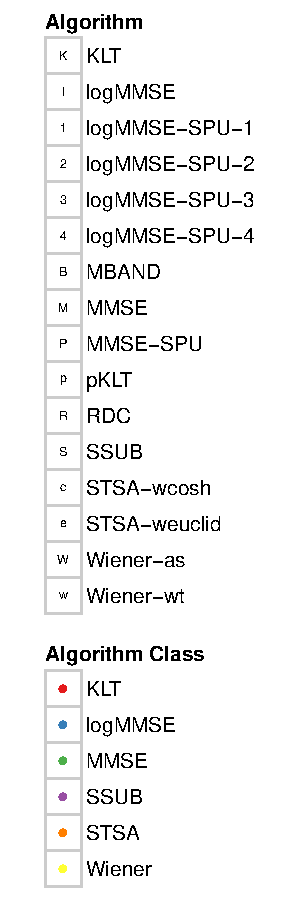
\includegraphics[width=0.2\textwidth]{fig/R/dir/lit/HumanMachineAllLegend}

}\protect\caption{\label{fig:Direct-PESQ-PRR}Direct comparison of human (\acs{PESQ})
vs. machine (\acs{PRR}) quality improvement}
\end{figure}


Shown in \figref{Group-PESQ-PRR} are the results of the group comparison,
a method also outlined in \subsecref{Method-Existing-Data}.

\begin{figure}[p]
\subfloat[\label{fig:Group-PESQ-PRR-LOESS}\acs{LOESS} fit]{\includegraphics[width=1\textwidth]{\string"fig/R/dir/lit/ HumanMachineGroupedLOESS\string".pdf}

}

\subfloat[\label{fig:Group-PESQ-PRR-LM}\acs{LM} fit]{\includegraphics[width=1\textwidth]{\string"fig/R/dir/lit/ HumanMachineGroupedLM\string".pdf}

}\protect\caption{\label{fig:Group-PESQ-PRR}Grouped comparison of human (\acs{PESQ})
vs. machine (\acs{PRR}) quality improvement}
\end{figure}


Results outlined in \tabref{LF-Fit-Direct-Compar-PESQ-PRR} are the
coefficients relating to the \ac{LM} fitted lines in \figref{Group-PESQ-PRR-LM}.

\begin{table}[h]
\protect\caption{\label{tab:LF-Fit-Direct-Compar-PESQ-PRR}Summary of \acs{LM} fit
($y=mx+c$) of direct comparison of \acs{PESQ} vs. \acs{PRR} improvement}


\centering\csvautotabular{dat/HumanMachinePaliwal.csv}
\end{table}


Additionally, a Pearson's correlation table was formed over a number
of the evaluation measures, depicted in the correlogram in \figref{litResCorr}.
The correlogram shows the Pearson correlation with confidence intervals
in the lower panels and a scatterplot in the upper panels. The sparsity
in this figure is due to the limited amount of pre-existing data.

\begin{figure}[h]
\noindent \begin{centering}
\includegraphics[width=1\textwidth]{fig/R/cor/litResCorrgram}
\par\end{centering}

\protect\caption{\label{fig:litResCorr}Pearson's correlation over some of the evaluation
measures assessed in existing data}
\end{figure}


\clearpage{}


\subsection{Independent Investigation}

The algorithms listed in \nameref{tab:Algorithms} were implemented,
as were the the evaluation measured outline in \subsecref{Independent-Investigation-Meth}.
A correlogram of the results was formed in \figref{my-Corr} to give
an overview of the results and how measures correlated with one another.
In this figure:
\begin{itemize}
\item the utterances and phonemes rows/columns correspond to the training
given to the enhancement algorithm;
\item ``Imp'' refers to improvement comparatively with the signal before
enhancement, i.e., pesqImp refers to the \ac{PESQ} score after enhancement
minus the \ac{PESQ} score before enhancement;
\item MOSle refers to the \ac{MOS} listening effort scale \citep{InternationalTelecommunicationUnion1996};
\item CMOS refers to the comparative \ac{MOS};
\item PRRcorr refers to the \ac{PRR} measured as the percentage correct;
and
\item PRRacc refers the the \ac{PRR} measures as the accuracy, defined
as the number of correct phonemes minus the number of insersions divided
by the number of phonemes.
\end{itemize}
The results of the \ac{PESQ} evaluation are given in \Cref{fig:my-PESQ,fig:my-PESQ-imp,fig:my-segSNR,fig:my-segSNR-imp,fig:my-PRRcorr,fig:my-MOS,fig:my-MOSle,fig:my-CMOS,fig:my-PRRcorr-imp,fig:my-PRRacc,fig:my-PRRacc-imp}.
These plots also show box plots of the five-point summaries of the
results. These results were used in investigating the correlation
between \ac{HR} and \ac{MR} and also to assess the performance of
the proposed changes to the enhancement algorithms outlined in \secref{Develop-Phoneme-Dependent}.
The changes proposed in \subsecref{Phoneme-Training} are implemented
in the algorithms \lstinline[breaklines=true]!phonemeIDBM!, \lstinline[breaklines=true]!phonemeMMSE!,
\lstinline[breaklines=true]!phonemeMohammadiaOnline! and \lstinline[breaklines=true]!phonemeMohammadiaSupervised!.
The changes proposed in \subsecref{Phoneme-Base} are implemented
in the algorithms \lstinline[breaklines=true]!phonemeModifiedOnline!
and \lstinline[breaklines=true]!phonemeModifiedSupervised!.


\subsubsection*{Observations}

In performing these tests a number of observations were also made.

It was noted that the ideal binary mask algorithms often caused the
the signals to be reduced to near silence. Especially during the \ac{MOS}
tests, where it was noted that most participants complained that occasionally
a signal would not play. Upon further investigation it was determined
the signal was in fact playing, and that the signal consisted of silence.
Subjects were instructed to continue answering the questions as they
were worded, and thus these signals were given the minimum scores.
This is reflected in \Cref{fig:my-MOS,fig:my-MOSle,fig:my-CMOS},
where the ideal binary mask algorithms scored poorly.

\begin{figure}[h]
\noindent \begin{centering}
\includegraphics[width=1\textwidth]{fig/R/dir/my/corr}
\par\end{centering}

\protect\caption{\label{fig:my-Corr}\foreignlanguage{australian}{Correlogram of results
of independent investigation}\selectlanguage{australian}%
}
\end{figure}


\begin{figure}[p]
\noindent \begin{centering}
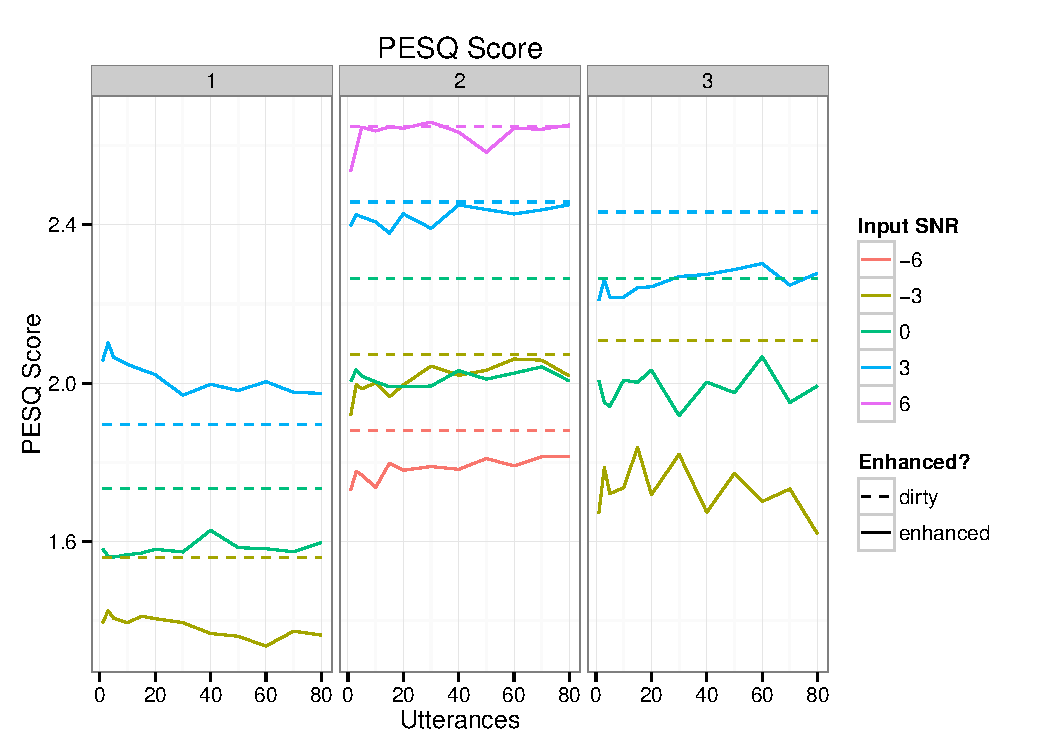
\includegraphics[angle=90,width=1\textwidth,height=0.95\textheight]{fig/R/my/pesq}
\par\end{centering}

\protect\caption{\label{fig:my-PESQ}\foreignlanguage{australian}{\acs{PESQ} results
of independent investigation}\selectlanguage{australian}%
}
\end{figure}


\begin{figure}[p]
\noindent \begin{centering}
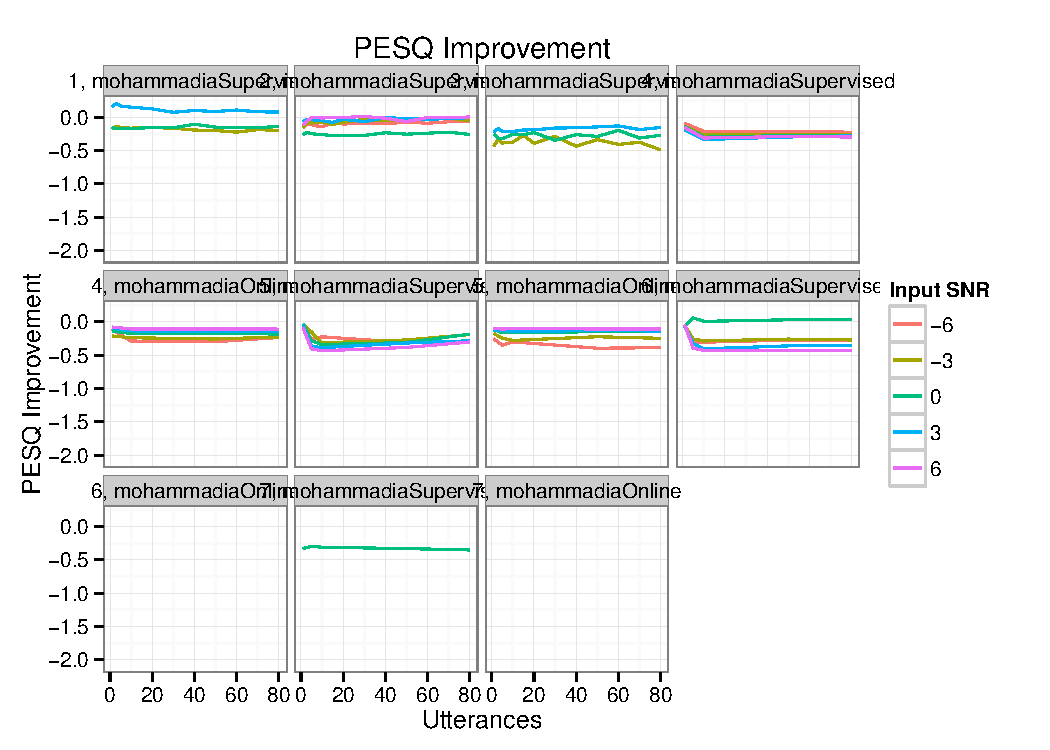
\includegraphics[angle=90,width=1\textwidth,height=0.95\textheight]{fig/R/my/pesqImp}
\par\end{centering}

\protect\caption{\label{fig:my-PESQ-imp}Improvement in \foreignlanguage{australian}{\acs{PESQ}
score due to enhancement}\selectlanguage{australian}%
}
\end{figure}


\begin{figure}[h]
\noindent \begin{centering}
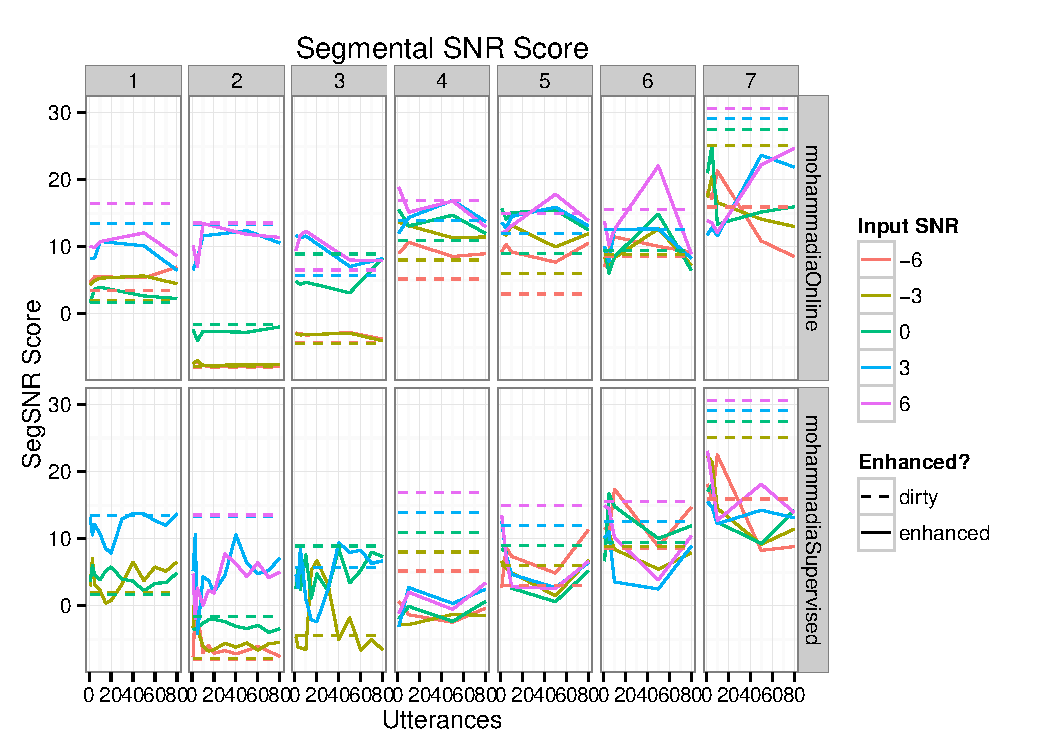
\includegraphics[angle=90,width=1\textwidth,height=0.95\textheight]{fig/R/my/segSNR}
\par\end{centering}

\protect\caption{\label{fig:my-segSNR}Segmental \foreignlanguage{australian}{\acs{SNR}
results of independent investigation}\selectlanguage{australian}%
}
\end{figure}


\begin{figure}[h]
\noindent \begin{centering}
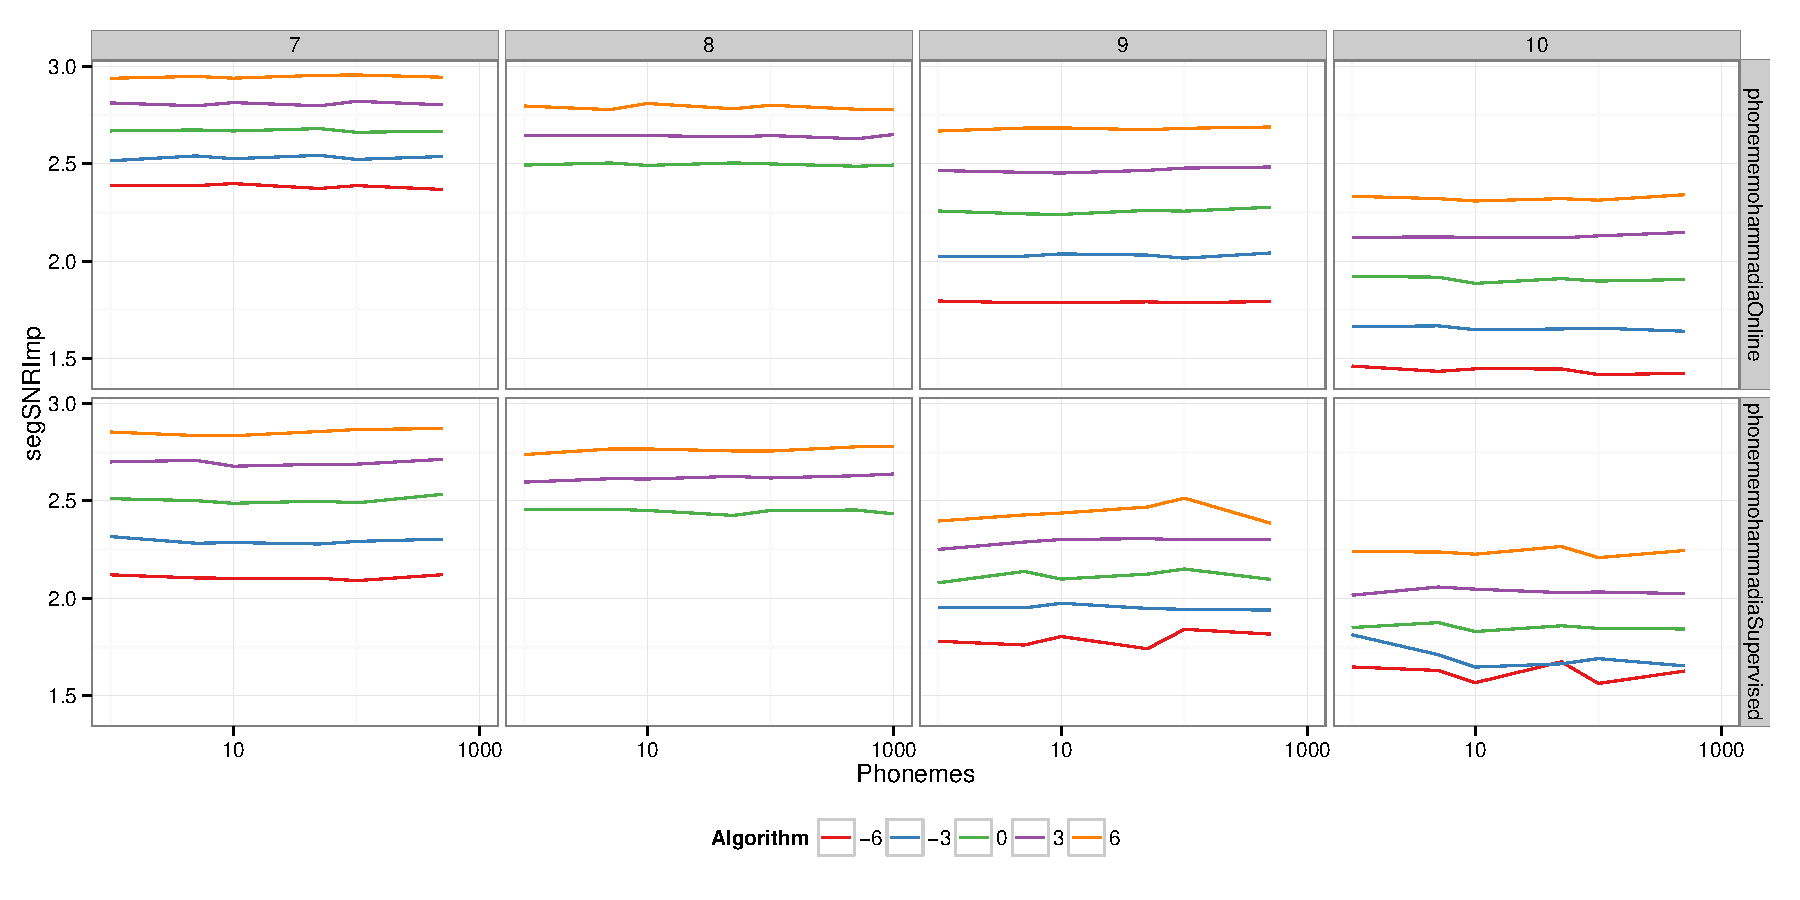
\includegraphics[angle=90,width=1\textwidth,height=0.95\textheight]{fig/R/my/segSNRImp}
\par\end{centering}

\protect\caption{\label{fig:my-segSNR-imp}Improvement in segmental \foreignlanguage{australian}{\acs{SNR}
score due to enhancement}\selectlanguage{australian}%
}
\end{figure}


\begin{figure}[h]
\noindent \begin{centering}
\includegraphics[angle=90,width=1\textwidth,height=0.95\textheight,keepaspectratio]{fig/R/my/MOS}
\par\end{centering}

\protect\caption{\label{fig:my-MOS}\foreignlanguage{australian}{\acs{MOS} results
of independent investigation}\selectlanguage{australian}%
}
\end{figure}


\begin{figure}[h]
\noindent \begin{centering}
\includegraphics[angle=90,width=1\textwidth,height=0.95\textheight,keepaspectratio]{fig/R/my/MOSle}
\par\end{centering}

\protect\caption{\label{fig:my-MOSle}Listening effort \foreignlanguage{australian}{\acs{MOS}
results of independent investigation}\selectlanguage{australian}%
}
\end{figure}


\begin{figure}[h]
\noindent \begin{centering}
\includegraphics[angle=90,width=1\textwidth,height=0.95\textheight,keepaspectratio]{fig/R/my/CMOS}
\par\end{centering}

\protect\caption{\label{fig:my-CMOS}Comparative \foreignlanguage{australian}{\acs{MOS}
results of independent investigation}\selectlanguage{australian}%
}
\end{figure}


\begin{figure}[h]
\noindent \begin{centering}
\includegraphics[angle=90,width=1\textwidth,height=0.95\textheight,keepaspectratio]{fig/R/my/PRRcorr}
\par\end{centering}

\protect\caption{\label{fig:my-PRRcorr}\foreignlanguage{australian}{\acs{PRR} correctness
results of independent investigation}\selectlanguage{australian}%
}
\end{figure}


\begin{figure}[h]
\noindent \begin{centering}
\includegraphics[angle=90,width=1\textwidth,height=0.95\textheight,keepaspectratio]{fig/R/my/PRRcorrImp}
\par\end{centering}

\protect\caption{\label{fig:my-PRRcorr-imp}Improvement in \foreignlanguage{australian}{\acs{PRR}
correctness due to enhancement}\selectlanguage{australian}%
}
\end{figure}


\begin{figure}[h]
\noindent \begin{centering}
\includegraphics[angle=90,width=1\textwidth,height=0.95\textheight,keepaspectratio]{fig/R/my/PRRacc}
\par\end{centering}

\protect\caption{\label{fig:my-PRRacc}\foreignlanguage{australian}{\acs{PRR} accuracy
results of independent investigation}\selectlanguage{australian}%
}
\end{figure}


\begin{figure}[h]
\noindent \begin{centering}
\includegraphics[angle=90,width=1\textwidth,height=0.95\textheight,keepaspectratio]{fig/R/my/PRRaccImp}
\par\end{centering}

\protect\caption{\label{fig:my-PRRacc-imp}Improvement in \foreignlanguage{australian}{\acs{PRR}
accuracy due to enhancement}\selectlanguage{australian}%
}
\end{figure}


\clearpage{}


\section{Assessing \acl{NMF} Algorithm Training}

The following are the results of investigations attempting to answer
Research Question \ref{enu:ResQ2}, \textit{\RQtwo{}}


\subsection{Investigating Training Requirements}

The results of the experiments proposed in \subsecref{Investigating-Training-Req}
are given in this section. \figref{vary-train-pesq} shows the \ac{PESQ}
results of the \ac{BNMF} algorithm developed by \citet{mohammadiha2013supervised}.
\figref{vary-train-pesq-imp} shows the \ac{PESQ} improvement as
compared to the dirty signal before enhancement. Similarly, \figref{vary-train-segsnr}
shows the segmental \ac{SNR} results of the same algorithm, and \figref{vary-train-segsnr-imp}
shows the segmental \ac{SNR} improvement compared against the signal
before enhancement.

Plots in \Cref{fig:vary-train-pesq,fig:vary-train-pesq-imp,fig:vary-train-segsnr,fig:vary-train-segsnr-imp}
each are arranged with the number of trained utterances on the x-axis
and test score on the y-axis. Furthermore, the plots are arranged
in a grid with rows corresponding to the enhancement algorithm and
columns corresponding to the test. Test labels give information on
the speaker ID and in brackets the sex of both the SoI, and the speakers
used to form the noise babble. Finally, series colour represents the
\ac{SNR} used for the test data, and the line type is dashed when
representing the score of the dirty signal before enhancement. The
R script used to form these plots is given in \lstref{trainReq}.

\figref{train-req-corr} shows a correlogram, an alternate view of
the same data. In the upper panels are scatter plots of each variable
pair. The lower panels are a heatmap of the Pearson's correlation
between the variables. Blue indicates a positive correlation, red
a negative, and the colour intensity indicates the magnitude.

\begin{figure}[p]
\noindent \begin{centering}
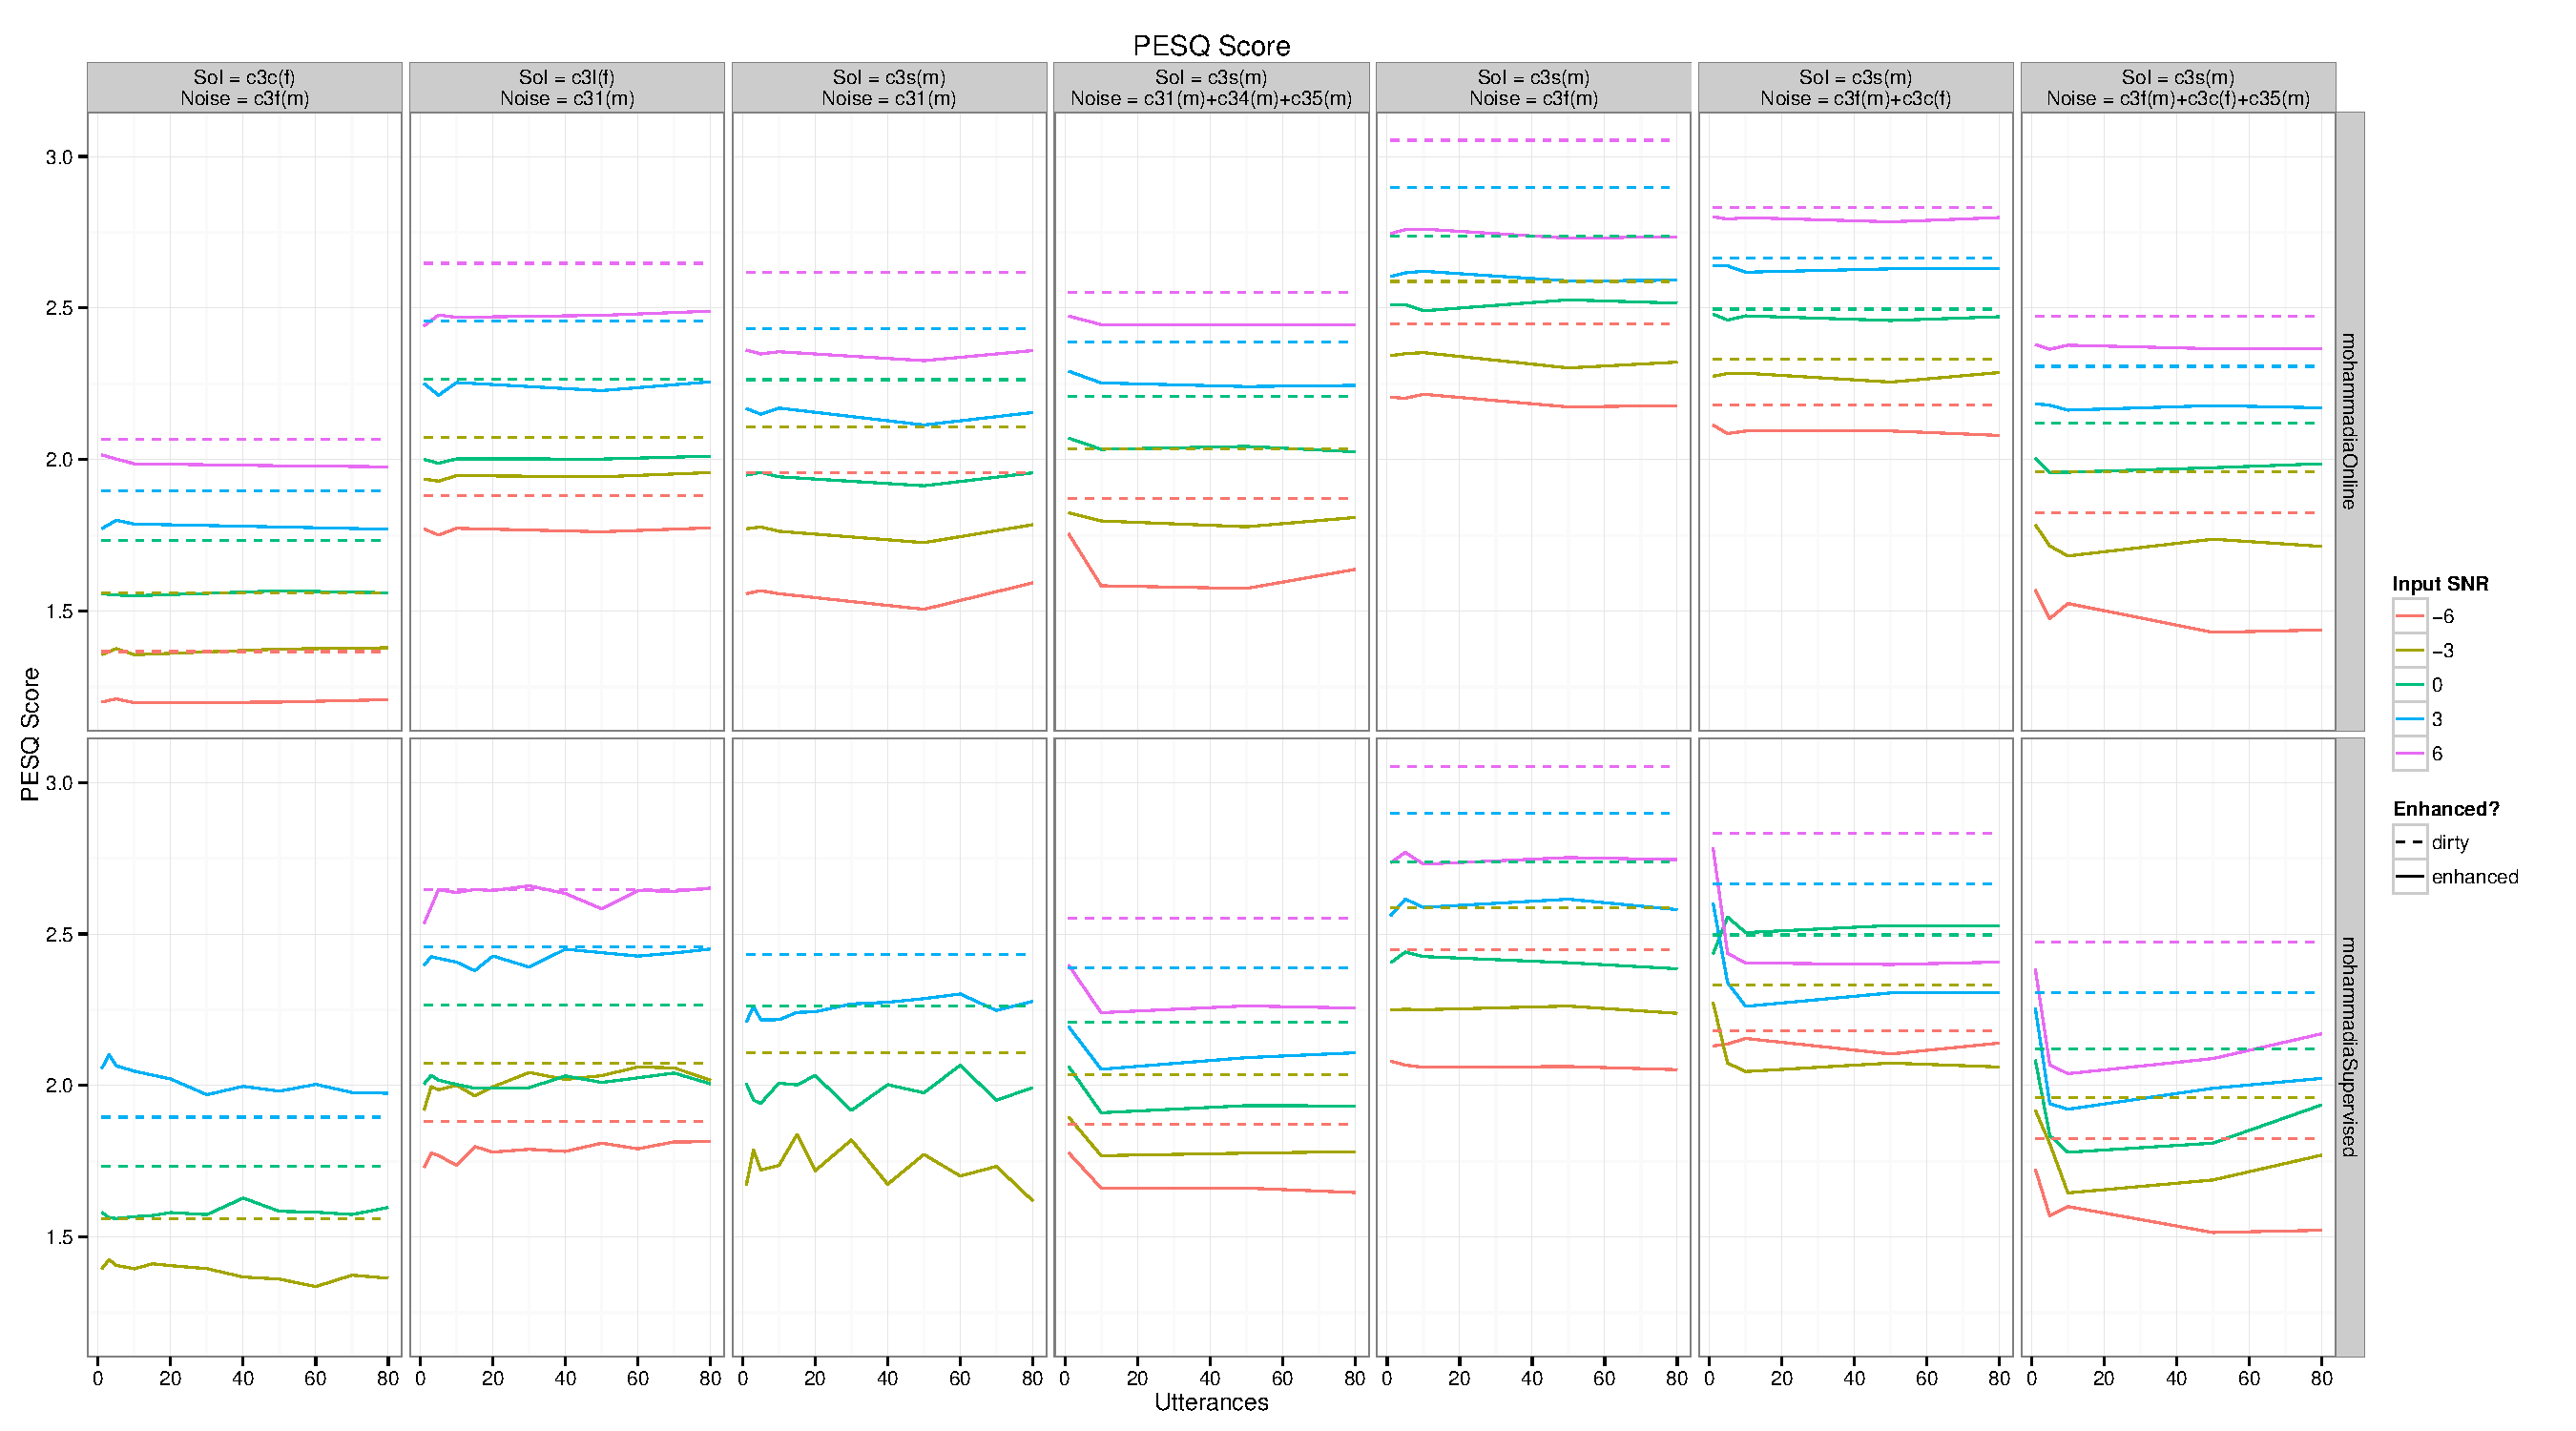
\includegraphics[angle=90,width=1\textwidth,height=0.95\textheight]{fig/R/train/pesq}
\par\end{centering}

\protect\caption{\label{fig:vary-train-pesq}\acs{PESQ} results of \acs{BNMF} algorithm
as training is increased}
\end{figure}


\begin{figure}[p]
\noindent \begin{centering}
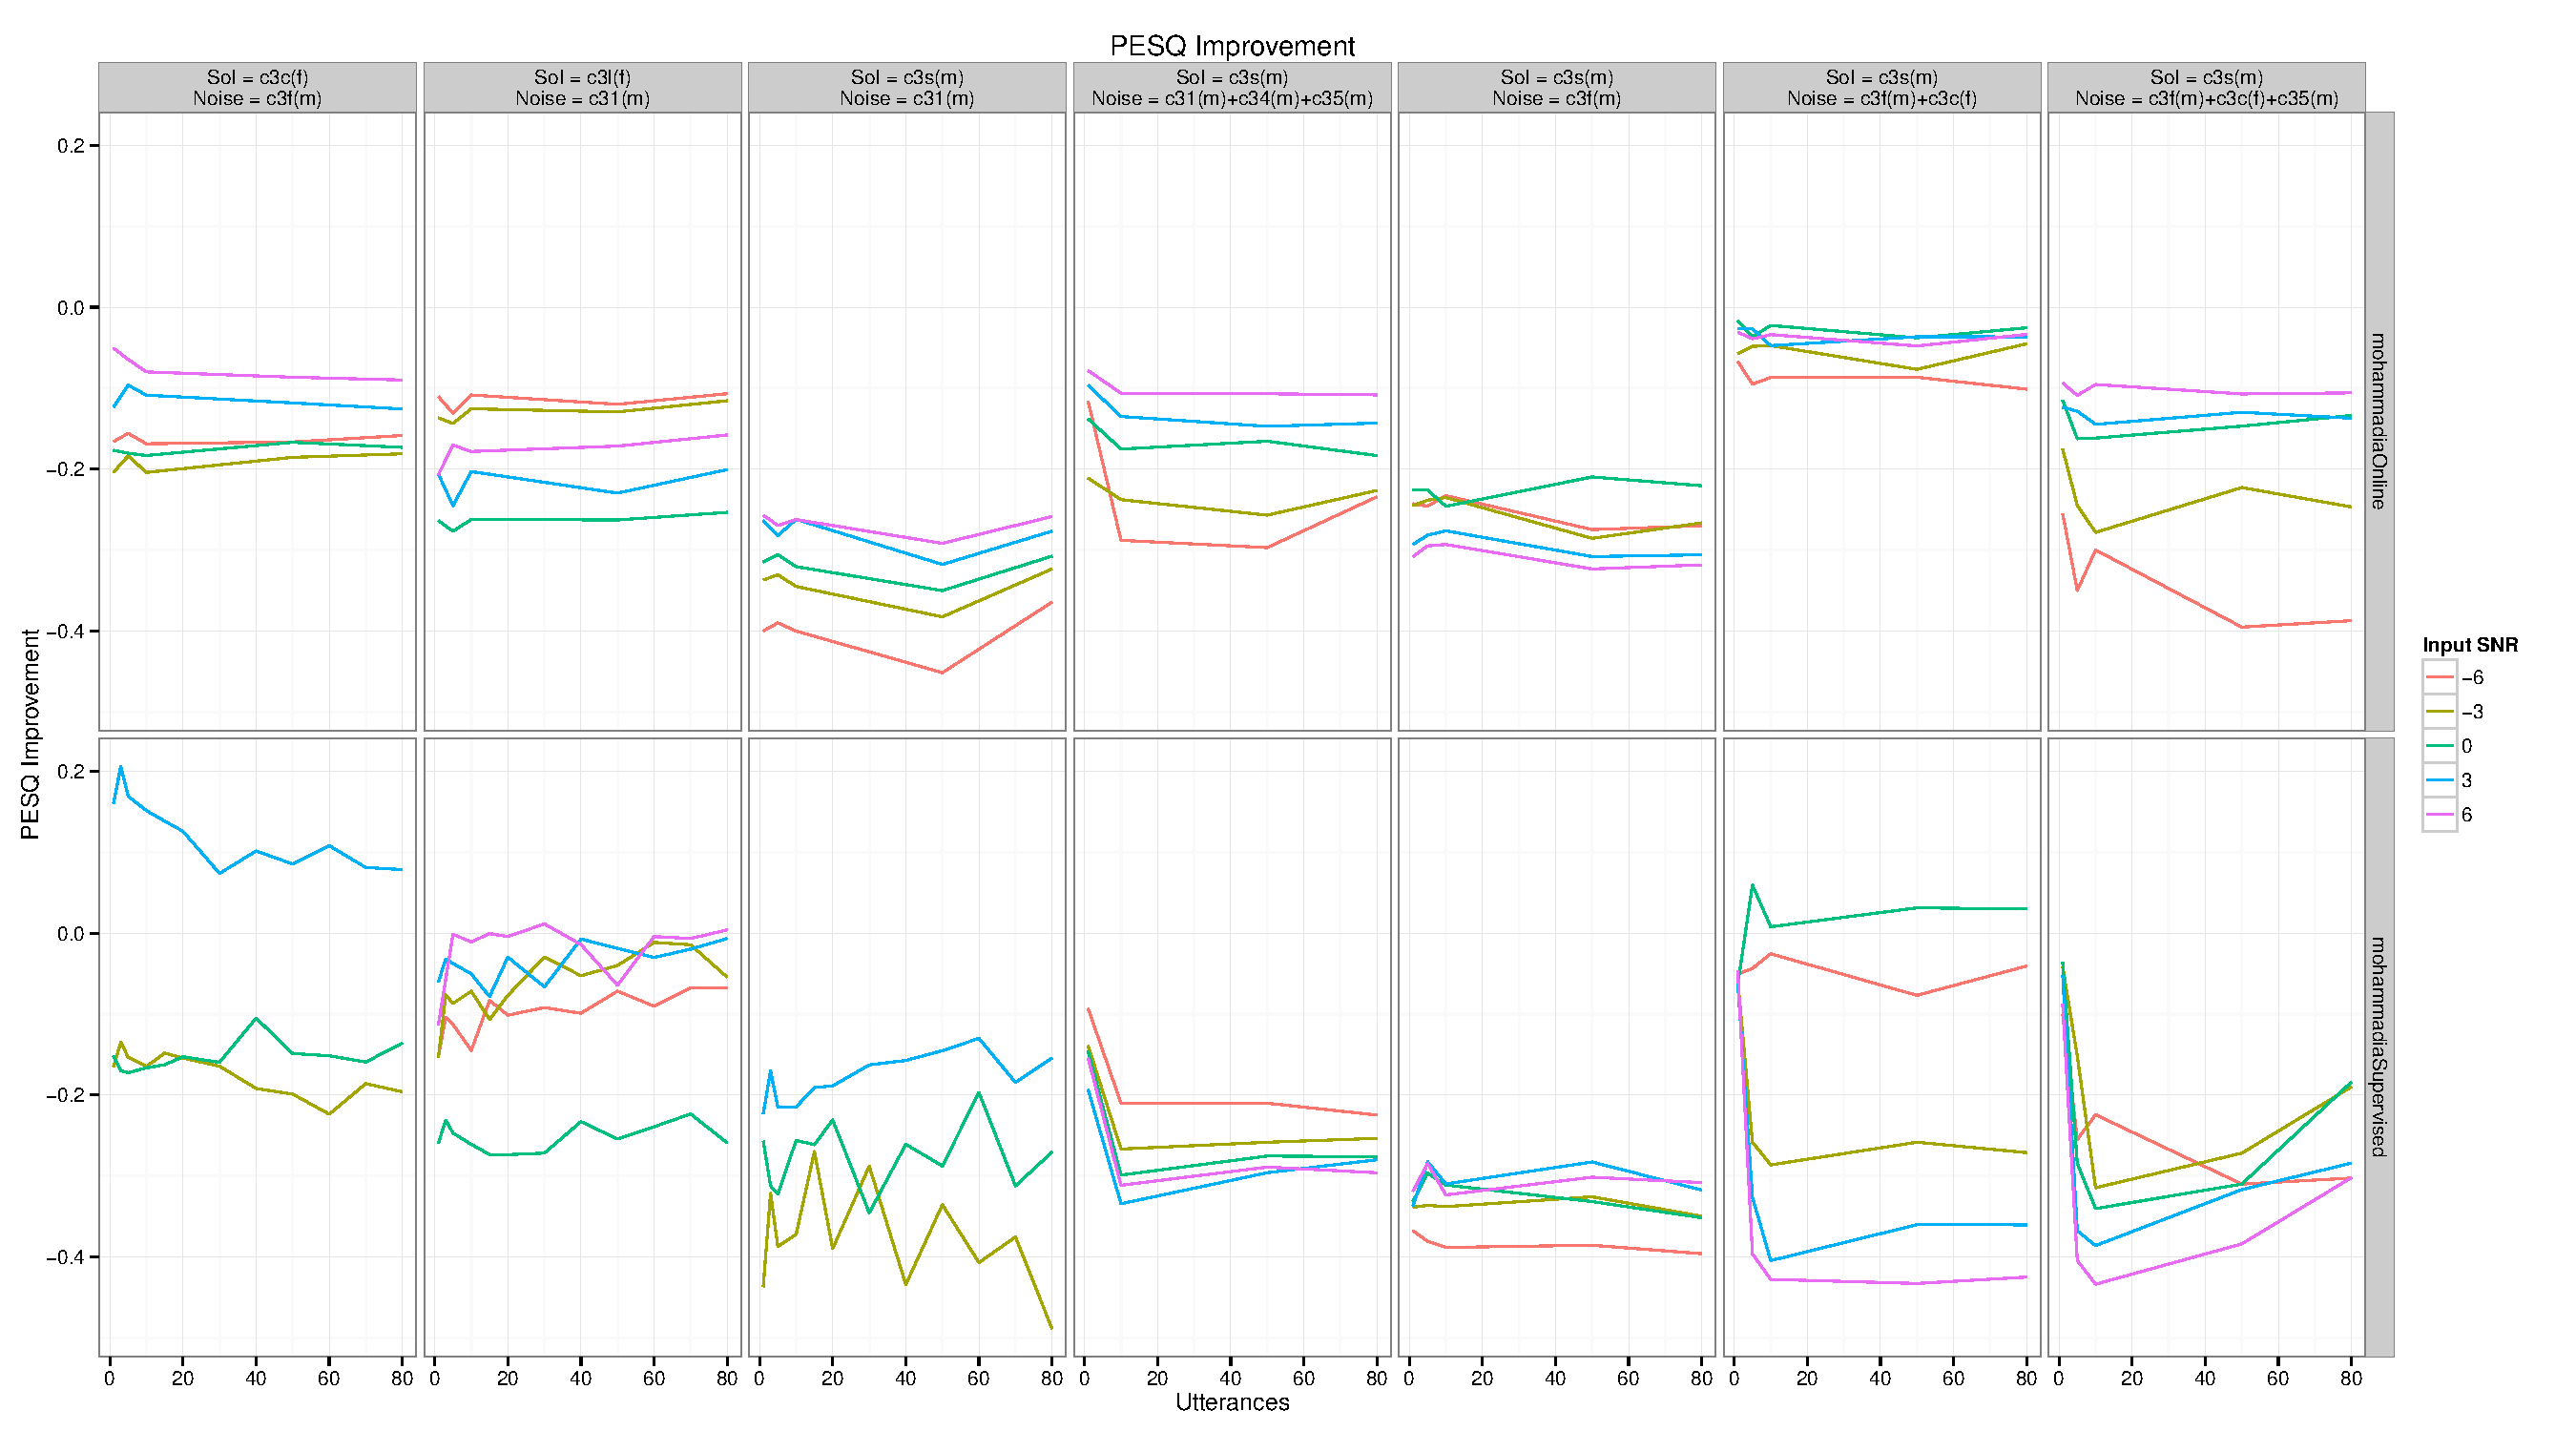
\includegraphics[angle=90,width=1\textwidth,height=0.95\textheight]{fig/R/train/pesqImp}
\par\end{centering}

\protect\caption{\label{fig:vary-train-pesq-imp}\acs{PESQ} improvement results of
\acs{BNMF} algorithm as training is increased}


\end{figure}


\begin{figure}[p]
\noindent \begin{centering}
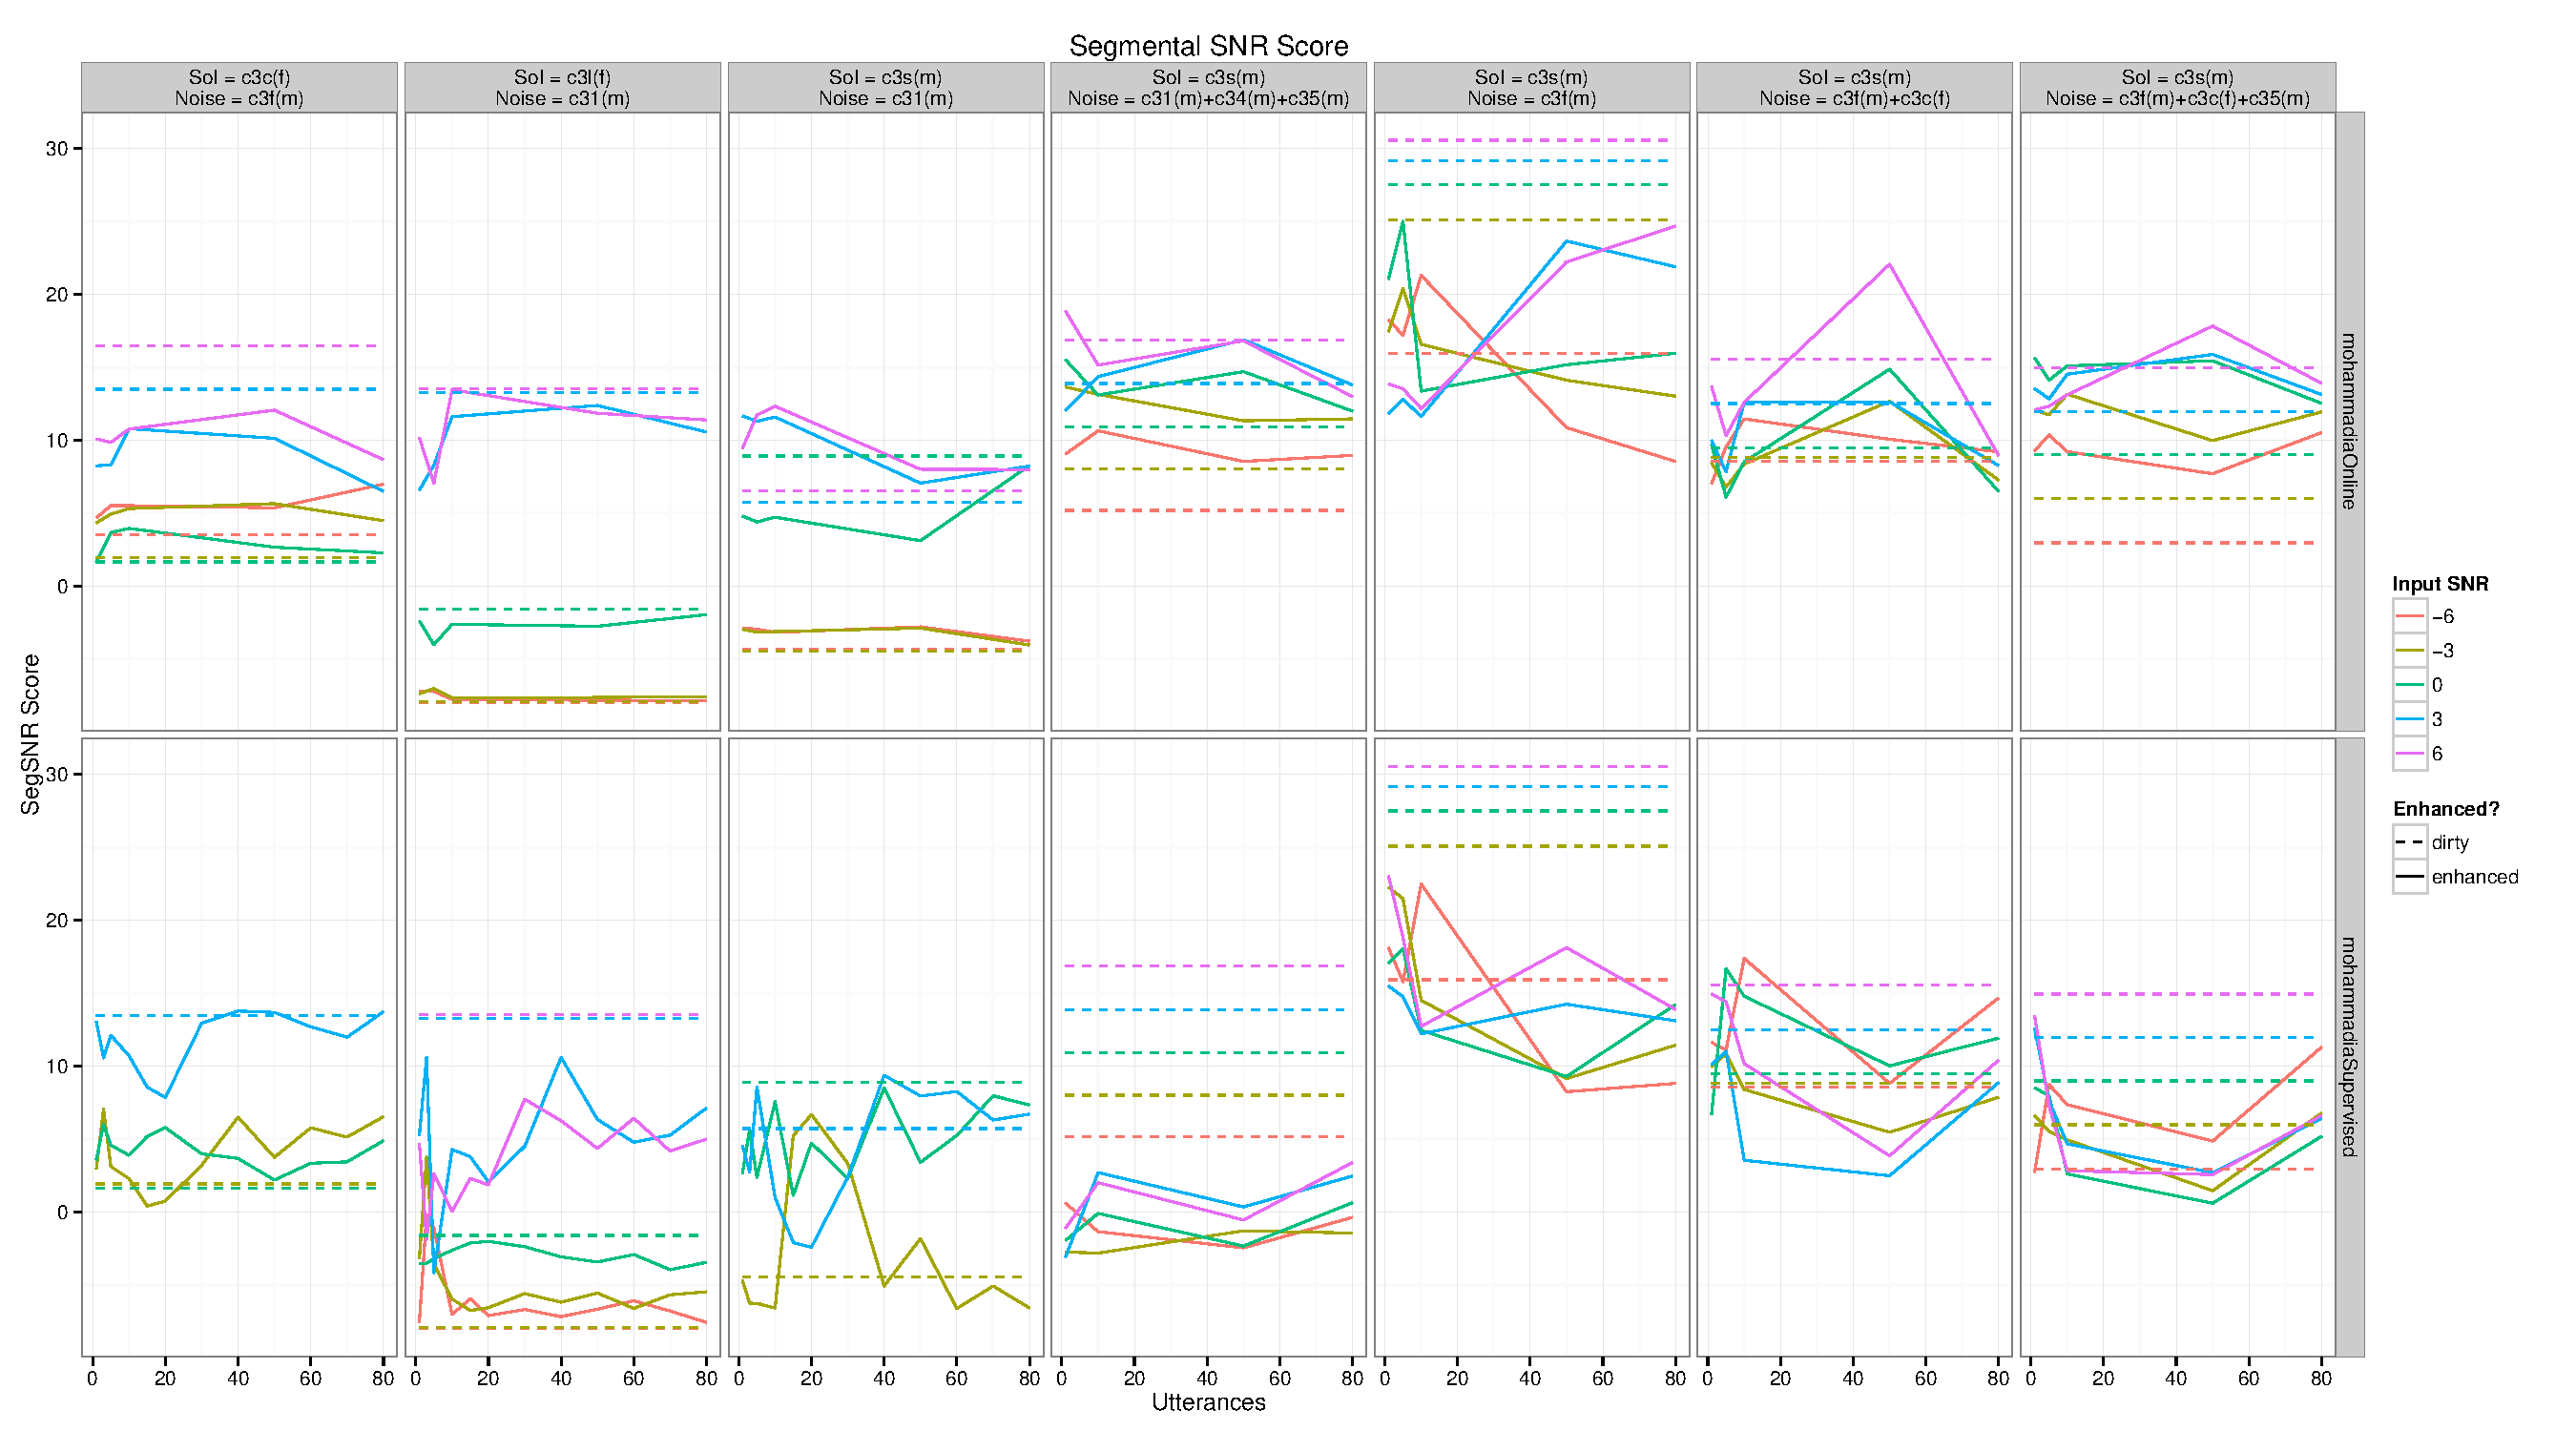
\includegraphics[angle=90,width=1\textwidth,height=0.95\textheight]{fig/R/train/segSNR}
\par\end{centering}

\protect\caption{\label{fig:vary-train-segsnr}Segmental \acs{SNR} results of \acs{BNMF}
algorithm as training is increased}
\end{figure}


\begin{figure}[p]
\noindent \begin{centering}
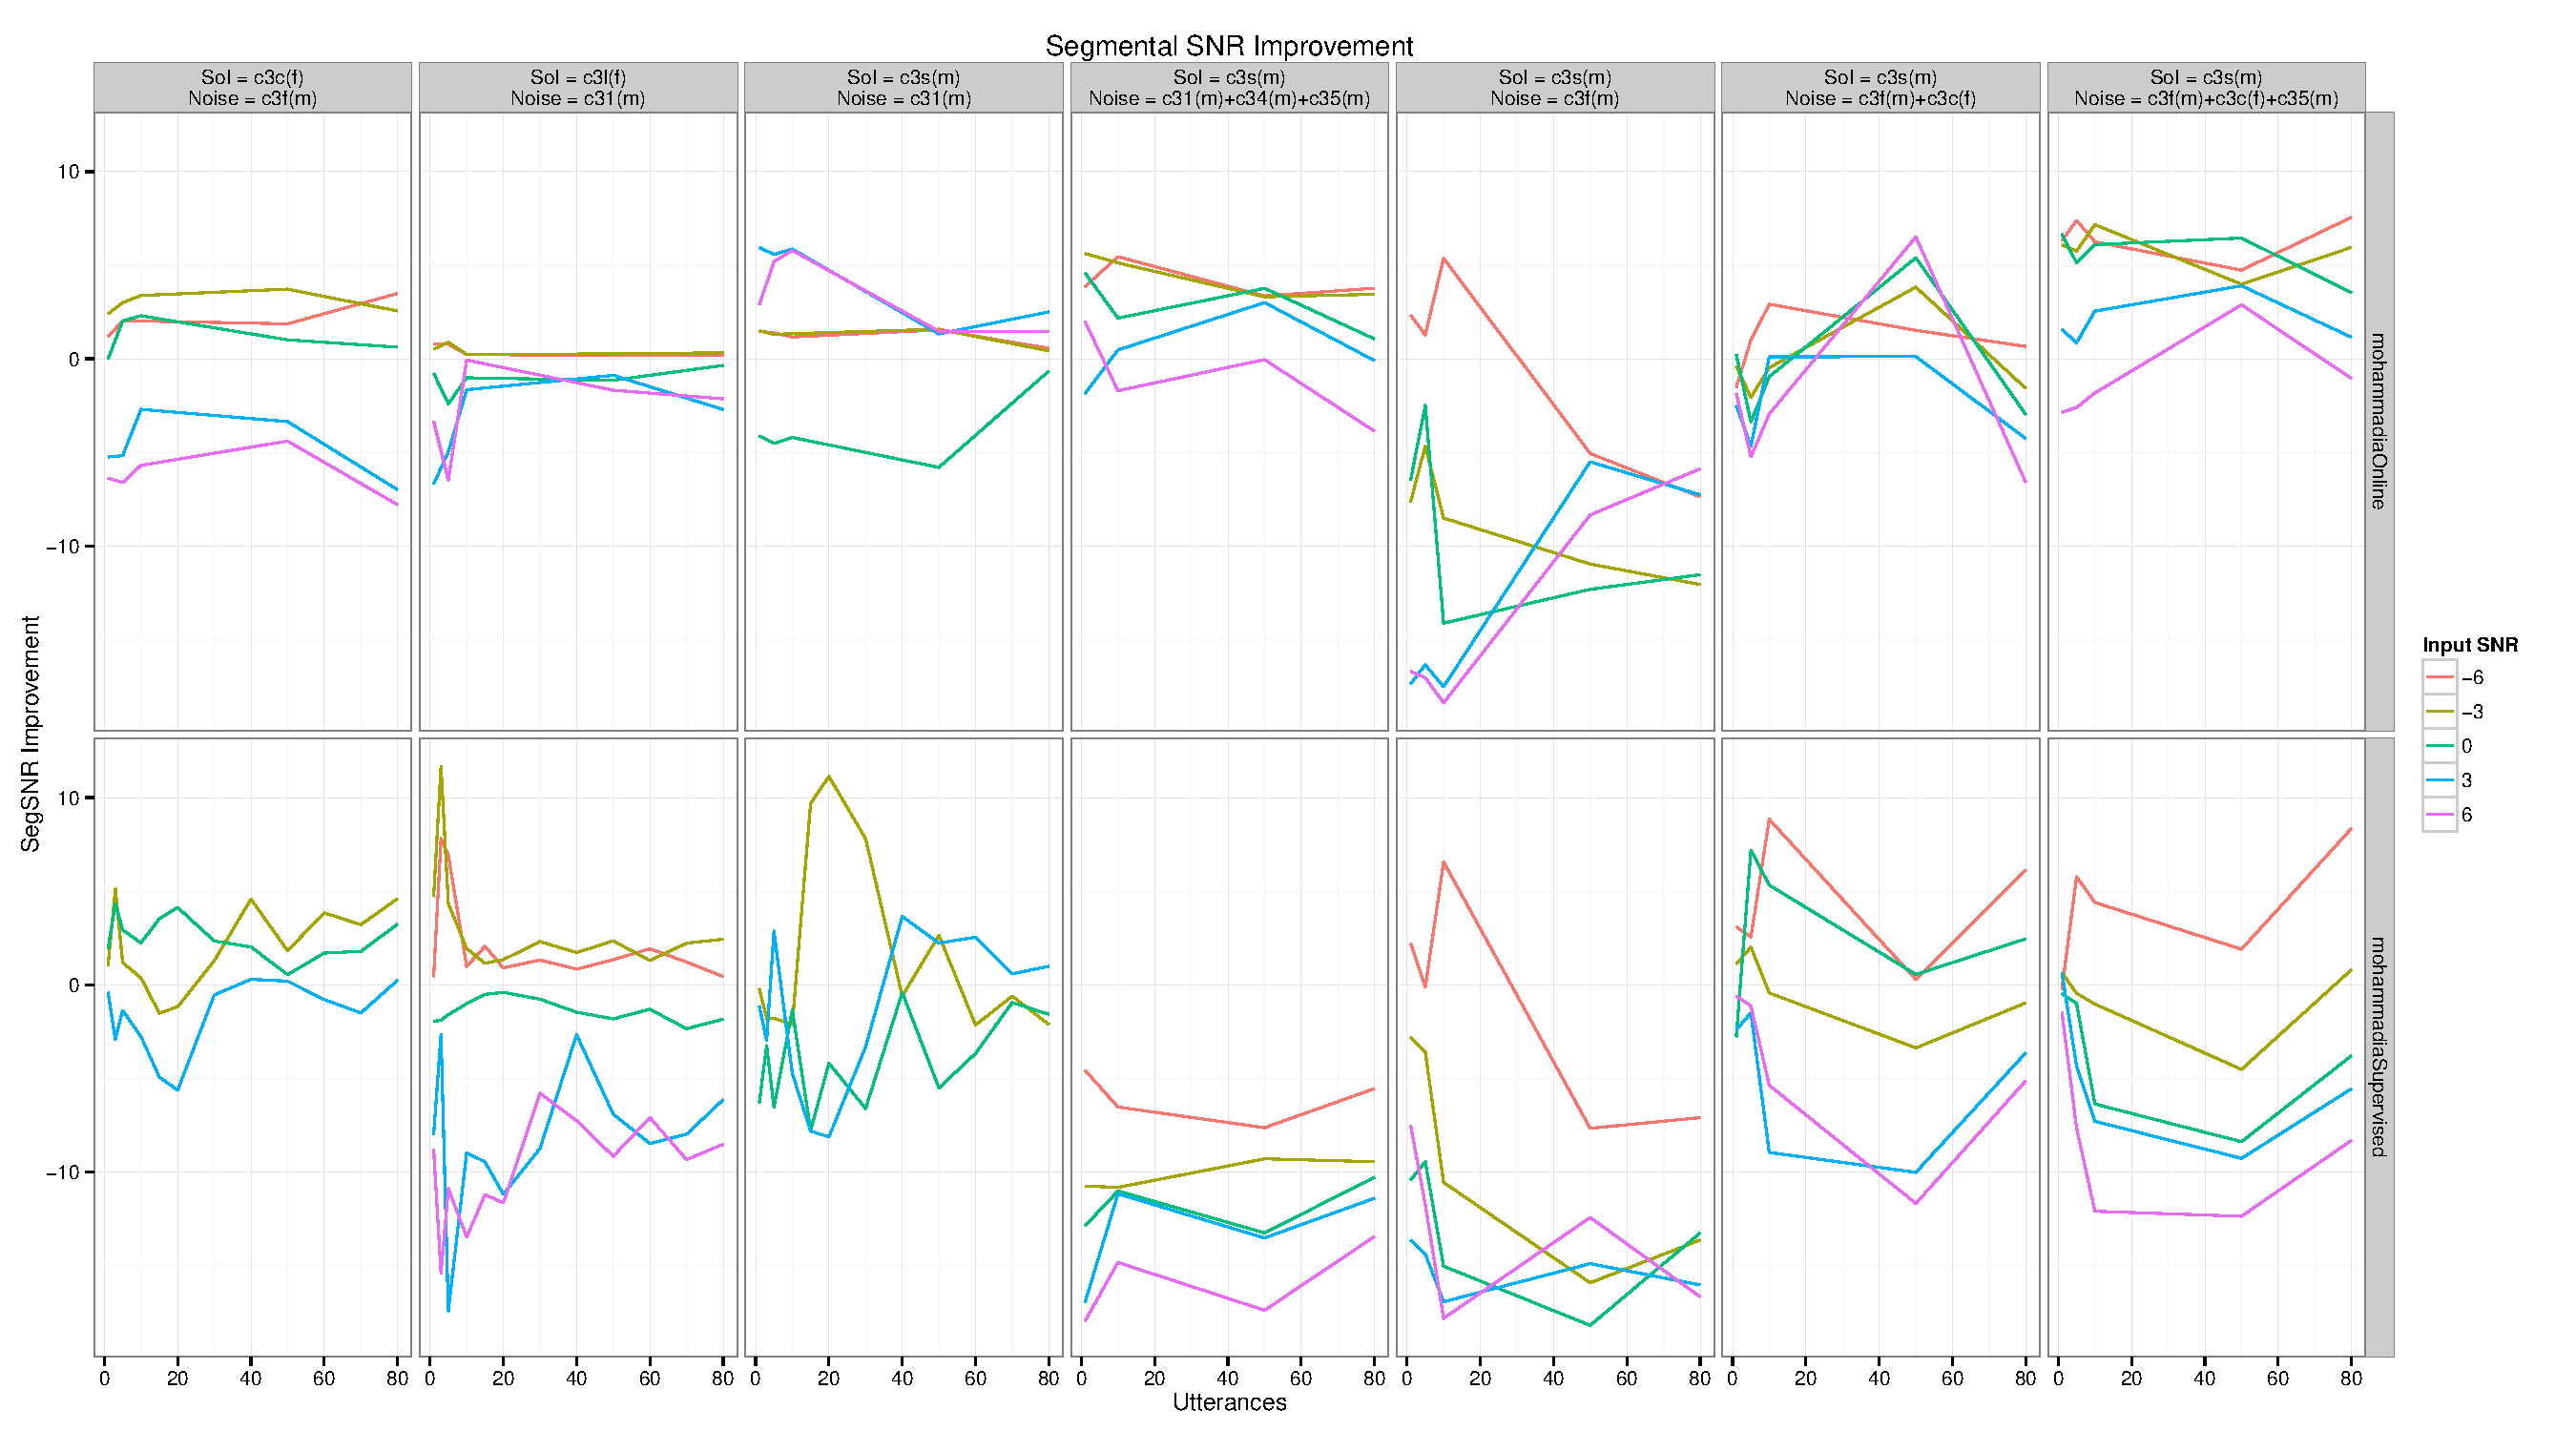
\includegraphics[angle=90,width=1\textwidth,height=0.95\textheight]{fig/R/train/segSNRImp}
\par\end{centering}

\protect\caption{\label{fig:vary-train-segsnr-imp}Segmental \acs{SNR} improvement
results of \acs{BNMF} algorithm as training is increased}
\end{figure}


\begin{figure}[h]


\noindent \begin{centering}
\includegraphics[width=0.9\textwidth]{fig/R/train/corr}
\par\end{centering}

\protect\caption{\label{fig:train-req-corr}Correlogram of results of training requirement
investigations}
\end{figure}


\clearpage{}


\section{Phoneme-Dependent Variation for the \acl{BNMF} Algorithm}

In order to force phoneme dependence in the algorithms to be modified,
phoneme samples first had to be formed. The phoneme sample recordings
were formed using the script in \lstref{createTestData}, with the
maximum number of samples drawn per phoneme varied. The length of
each sample drawn was $512/FS$, such that 256 frequency bins were
formed after taking the real \ac{FFT}. The typical spectrograms of
the drawn phonemes are given in \figref{drawn-phoneme-spectrogram},
showing the frequency characteristics of each phoneme.

\begin{figure}[h]
\subfloat[One sample per phoneme]{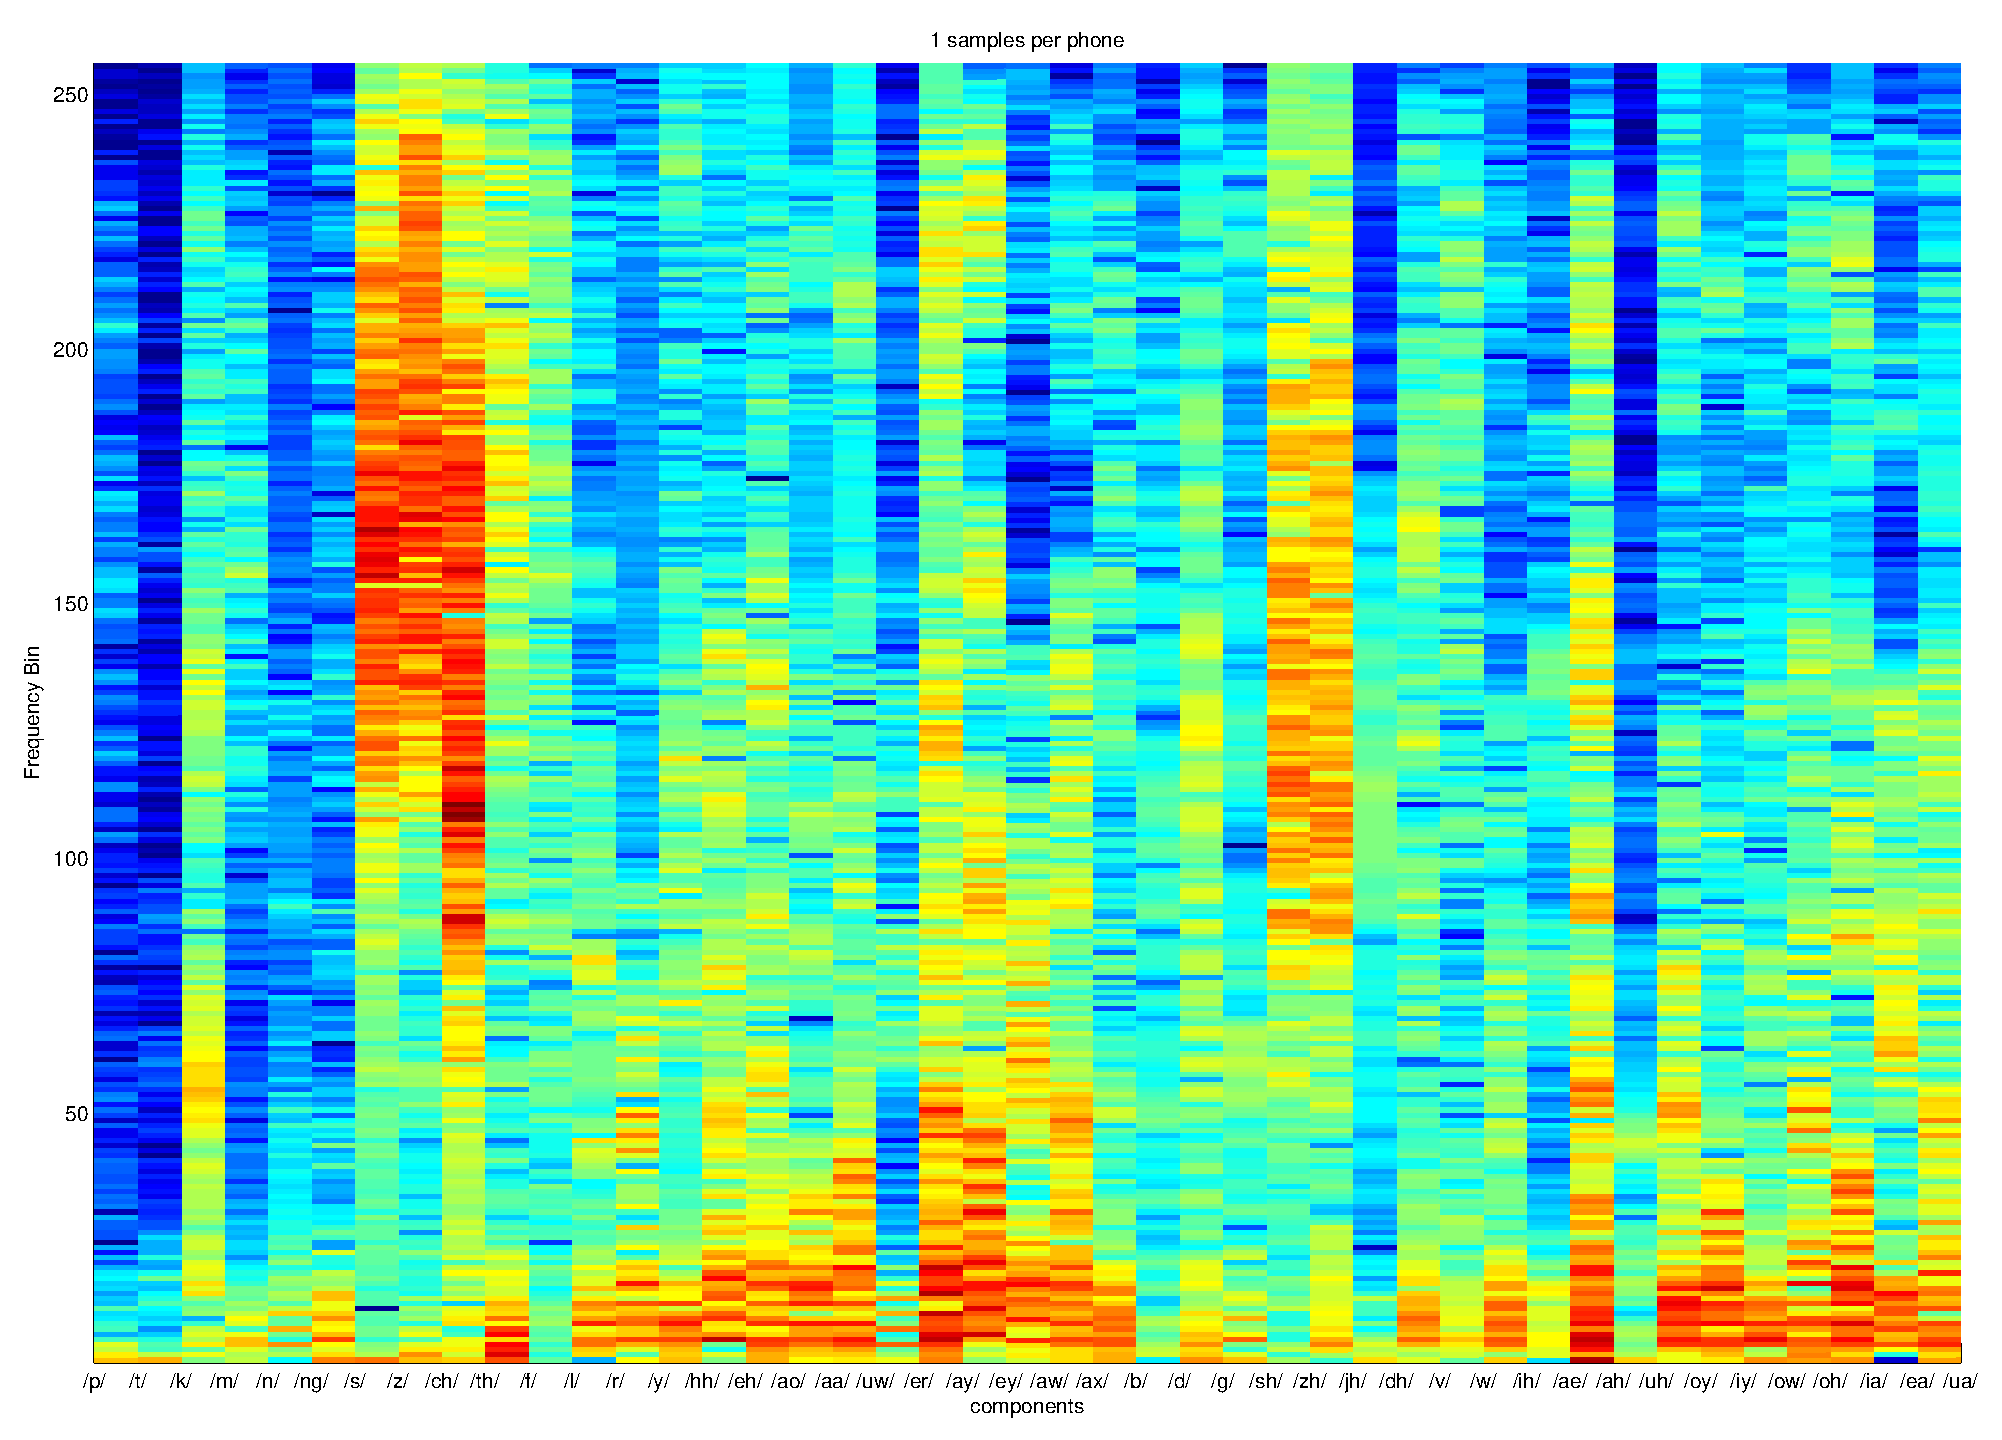
\includegraphics[width=0.5\textwidth]{fig/spectrogram/drawPhn/c3s-1phnSpectrogram}

}\subfloat[Five samples per phoneme]{

\includegraphics[width=0.5\textwidth]{fig/spectrogram/drawPhn/c3s-5phnSpectrogram}

}

\subfloat[Ten samples per phoneme]{\includegraphics[width=0.5\textwidth]{fig/spectrogram/drawPhn/c3s-10phnSpectrogram}

}\subfloat[50 samples per phoneme]{\includegraphics[draft,width=0.5\textwidth]{fig/spectrogram/drawPhn/c3s-50phnSpectrogram}

}

\subfloat[100 samples per phoneme]{\includegraphics[draft,width=0.5\textwidth]{fig/spectrogram/drawPhn/c3s-100phnSpectrogram}

}\subfloat[500 samples per phoneme]{\includegraphics[draft,width=0.5\textwidth]{fig/spectrogram/drawPhn/c3s-500phnSpectrogram}

}

\subfloat[999 samples per phoneme]{\includegraphics[draft,width=0.5\textwidth]{fig/spectrogram/drawPhn/c3s-999phnSpectrogram}

}

\protect\caption{\label{fig:drawn-phoneme-spectrogram}Typical spectrogram of randomly
drawn phoneme samples for speaker C3S}
\end{figure}



\subsection{Phoneme Dependent Training Data}

The following results relate to the proposed method outlined in \subsecref{Phoneme-Training}.


\subsection{Phoneme Dependent Base Matrix}

The first test conducted was to ensure the modifications to the code
indeed forced the \ac{NMF} spectral component matrix, \lstinline[language=Matlab]!Et!
in the \lstinline[language=bash]!NMF! class, to be the drawn phoneme
bases supplied.
